% !TeX root = ../main.tex
\documentclass[./../main.tex]{subfiles}

\begin{document}

\subsection{Kiểm thử đơn vị}

Trong quá trình phát triển, em đã viết các ca kiểm thử đơn vị để đảm bảo code hoạt động đúng như mong muốn. Hơn nữa, các ca kiểm thử đơn vị này sẽ được chạy lại mỗi khi mã nguồn được merge vào nhánh master, giúp cho các lỗi xảy ra khi kiểm thử có thể được phát hiện và sửa nhanh chóng hơn.

\begin{figure}[H]
	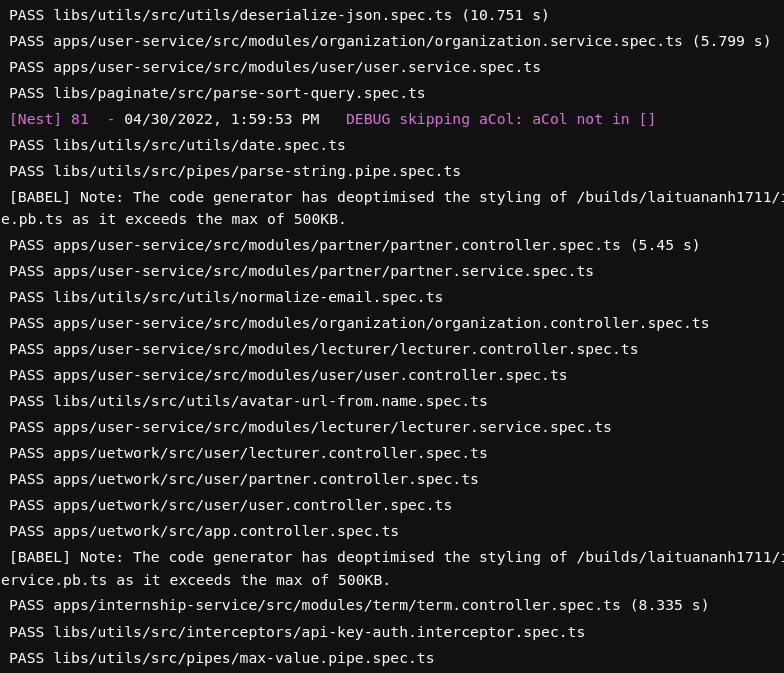
\includegraphics[width=\linewidth]{./images/image14.png}
	\caption{Kết quả kiểm thử đơn vị}
	\label{fig:unit_test_result}
\end{figure}

\subsection{Kiểm thử chức năng}

Phần này sẽ đưa ra một số ca kiểm thử chức năng đã được thực hiện và kết quả. Danh sách ca kiểm thử dưới đây có mục đích mô tả cách một ca kiểm thử được thực hiện và không bao gồm toàn bộ ca kiểm thử của hệ thống.

\subsubsection{Đăng nhập bằng email và mật khẩu (dữ liệu hợp lệ)}

\paragraph*{Bước kiểm thử}

\begin{enumerate}
    \item Người dùng truy cập vào trang đăng nhập.
    \item Người dùng nhập email và mật khẩu, sau đó chọn nút "Đăng nhập".
\end{enumerate}

\paragraph*{Dữ liệu kiểm thử} Email, mật khẩu

\paragraph*{Kết quả mong đợi} Người dùng được đưa tới trang chủ

\paragraph*{Kết quả thực tế} Như mong đợi

\paragraph*{Trạng thái} Đạt

\subsubsection{Đăng nhập bằng email và mật khẩu (sai email hoặc mật khẩu)}

\paragraph*{Bước kiểm thử}

\begin{enumerate}
    \item Người dùng truy cập vào trang đăng nhập.
    \item Người dùng nhập email và mật khẩu, sau đó chọn nút "Đăng nhập".
\end{enumerate}

\paragraph*{Dữ liệu kiểm thử} Email, mật khẩu

\paragraph*{Kết quả mong đợi}

\begin{itemize}
    \item Thông báo "sai email hoặc mật khẩu" được hiển thị
    \item Người dùng không được đưa tới trang chủ
\end{itemize}

\paragraph*{Kết quả thực tế} Như mong đợi

\paragraph*{Trạng thái} Đạt

\subsubsection{Đăng nhập bằng Google (dữ liệu hợp lệ)}

\paragraph*{Bước kiểm thử}

\begin{enumerate}
    \item Người dùng truy cập vào trang đăng nhập.
    \item Người dùng chọn "Đăng nhập bằng Google" và chọn tài khoản Google tương ứng
\end{enumerate}

\paragraph*{Dữ liệu kiểm thử} Tài khoản Google

\paragraph*{Kết quả mong đợi} Người dùng được đưa tới trang chủ

\paragraph*{Kết quả thực tế} Như mong đợi

\paragraph*{Trạng thái} Đạt

\subsubsection{Đăng nhập bằng Google (tài khoản không tồn tại trong hệ thống)}

\paragraph*{Bước kiểm thử}

\begin{enumerate}
    \item Người dùng truy cập vào trang đăng nhập.
    \item Người dùng chọn "Đăng nhập bằng Google" và chọn tài khoản Google
\end{enumerate}

\paragraph*{Dữ liệu kiểm thử} Tài khoản Google

\paragraph*{Kết quả mong đợi}

\begin{itemize}
    \item Thông báo "tài khoản không tồn tại" được hiển thị
    \item Người dùng không được đưa tới trang chủ
\end{itemize}

\paragraph*{Kết quả thực tế} Như mong đợi

\paragraph*{Trạng thái} Đạt

\subsubsection{Quên mật khẩu (dữ liệu hợp lệ)}

\paragraph*{Bước kiểm thử}

\begin{enumerate}
    \item Người dùng truy cập vào trang "Quên mật khẩu".
    \item Người dùng nhập email của tài khoản và chọn "Đặt lại mật khẩu".
\end{enumerate}

\paragraph*{Dữ liệu kiểm thử} Email của người dùng

\paragraph*{Kết quả mong đợi}

\begin{itemize}
    \item Thông báo gửi mail thành công được hiển thị
    \item Mail được gửi tới người dùng
\end{itemize}

\paragraph*{Kết quả thực tế} Như mong đợi

\paragraph*{Trạng thái} Đạt

\subsubsection{Chỉnh sửa thông tin cá nhân (dữ liệu hợp lệ)}

\paragraph*{Bước kiểm thử}

\begin{enumerate}
    \item Người dùng truy cập vào trang "Chỉnh sửa thông tin cá nhân".
    \item Người dùng chỉnh sửa thông tin cá nhân và chọn "Lưu thay đổi".
\end{enumerate}

\paragraph*{Dữ liệu kiểm thử} Thông tin cá nhân của người dùng (v.d. họ tên, số điện thoại, email, ...)

\paragraph*{Kết quả mong đợi}

\begin{itemize}
    \item Thông báo lưu thay đổi thành công được hiển thị
    \item Thông tin cá nhân của người dùng được lưu lại
\end{itemize}

\paragraph*{Kết quả thực tế} Như mong đợi

\paragraph*{Trạng thái} Đạt

\end{document}